%\section{Tutkimusaineisto ja -menetelmät}
\section{Antenna design objectives \& strategy}
\label{sec:ojectives}

\subsection{Antennas to design}
The objective of this thesis is to study feasible antenna structures for metal-covered mobile phones. The phone should have two similar cellular antennas (main and diversity) for MIMO operation. Additionally, an antenna for GPS and Wi-Fi is to be designed. Table \ref{tab:design_goals} below presents the goals and requirements for this project.

\begin{table}[H]
    \centering
    \caption{Criteria for the antennas to be designed.}
    \label{tab:design_goals}
    \begin{tabular}{|l|c|}
        \hline
         \textbf{Parameter} & \textbf{Value} \\
         \hline
         Reflection coefficient & $S_{11} < -5\,\db$\\
         \hline
         Total efficiency & $\eta > 30\,\%$\\
         \hline
         Isolation between main and diversity antenna & $S_{21} < -15\,\db$\\
         \hline\hline
         \textbf{Frequencies} & \\
         \hline
         Main cellular antenna & $0.704-0.960\,\giga\hertz, 1.71-2.69\,\giga\hertz$\\
         \hline
         Diversity cellular antenna & $0.704-0.960\,\giga\hertz, 1.71-2.69\,\giga\hertz$\\
         \hline
         GPS antenna & $1.56-1.61\,\giga\hertz$\\
         \hline
         Wi-Fi antenna & $2.4-2.484\,\giga\hertz, 5.15-5.875\,\giga\hertz$\\
         \hline
    \end{tabular}
\end{table}

\subsubsection{Model of the mobile phone}
\label{sec:phone}
\begin{itemize}
\item[--]dimensiot
\item[--]kriittiset osat
\item[--]mallin kehittyminen
\end{itemize}

\begin{figure}[H]
    \centering
    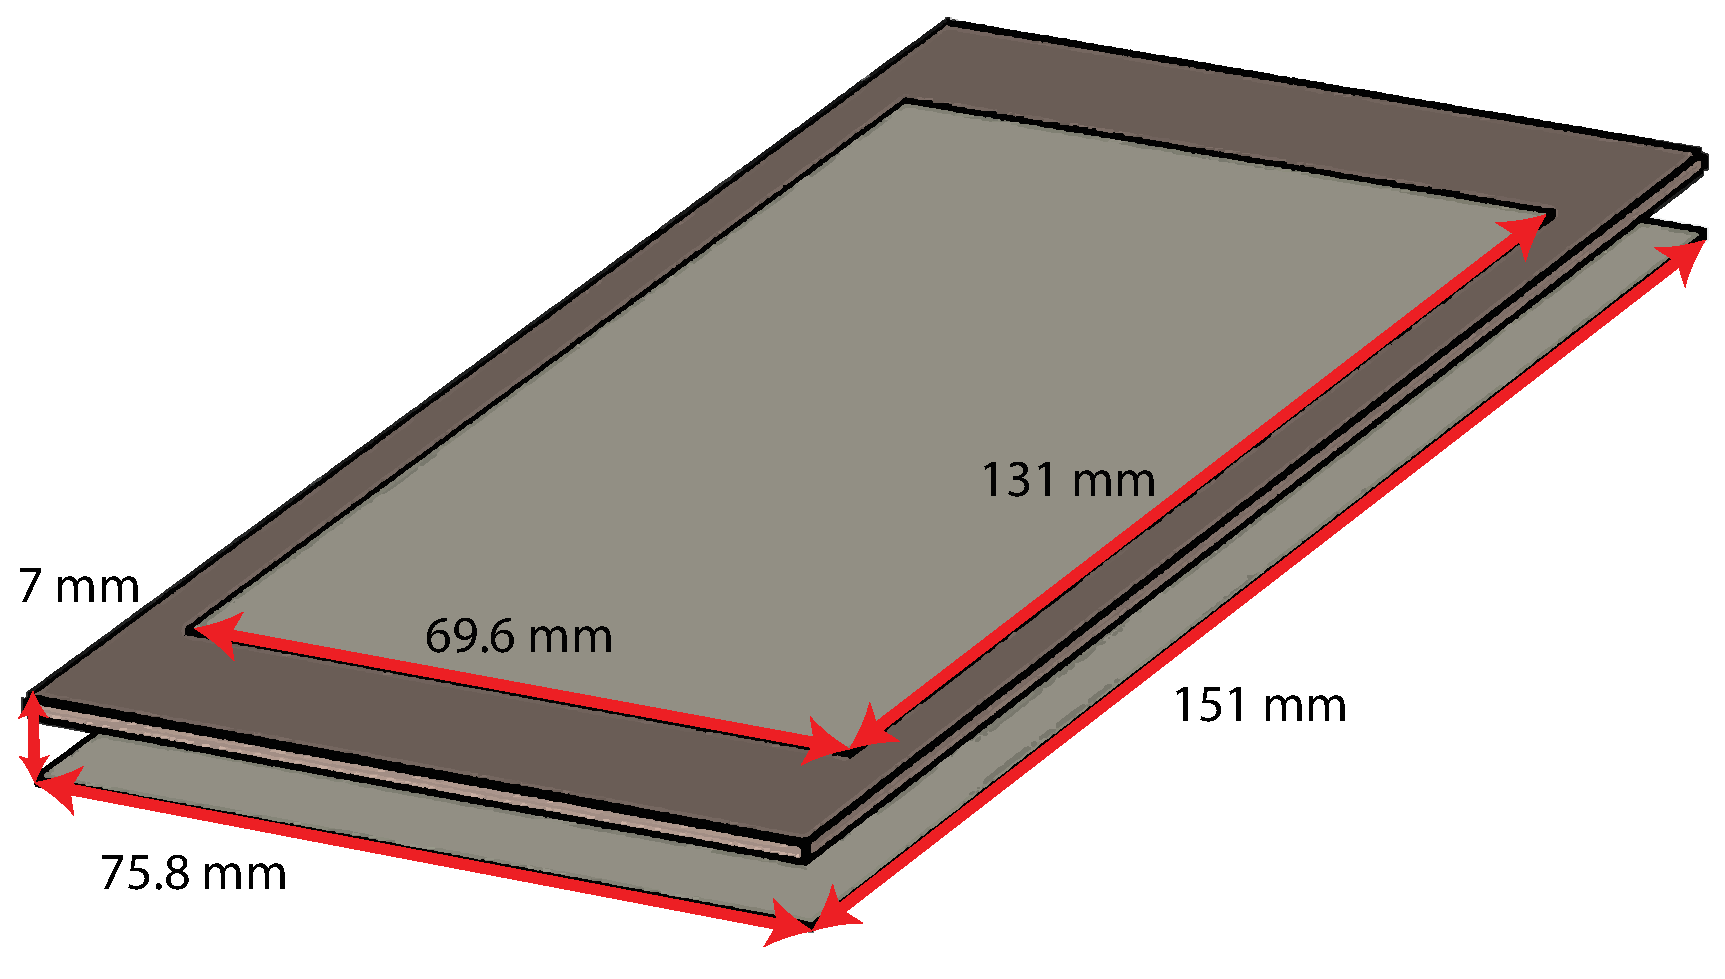
\includegraphics[width=0.6\textwidth]{img/basic_structure.eps}
    \caption{Simplified, basic model of a mobile phone to be used in simulations.}
    \label{fig:basic_structure}
\end{figure}



\subsection{Design strategy}
\label{sec:process}
Electromagnetic (EM) simulations were made in CST Microwave Studio \cite{cst}. It was used to create antenna and phone models and to calculate system's $S$-parameters. Simulations were focused on antenna's initial matching, i.e. $S_{11}$ for each antenna. The research strategy was first to find solution for the main antenna to operate on lower frequency band ($704-960\,\mega\hertz$). Lower band was designed first, since it is harder to reach the determined matching levels and efficiencies at lower frequencies. Results from previous studies have shown weaker performance at those frequencies. Also, the required antenna structures might be larger. After a reasonable performance was achieved at that band, model was configured to support also the upper frequencies ($1.71-2.69\,\giga\hertz$). When main antenna was operating properly, the same process was applied to design the diversity antenna. Final step was to add solutions for GPS and Wi-Fi antennas.

The procedure of testing different antenna structures was pretty straightforward: first a model was built, then simulated, and finally the obtained results were analyzed. Based on the previous findings, the model was modified aiming to wide impedance matching, and then simulated again. The first tests were done with a simple model and a simple antenna design. While the antenna structures got better, the model of the phone was also modified to be more realistic.

Designing antennas was not limited only in antenna structures. In order to reach the goals presented above, matching networks were to be designed as well. Finding usable circuit topologies was done simultaneously with EM simulations. Optenni Lab \cite{optenni} and NI AWR Design Environment \cite{awr} were used for that purpose. The $S$-parameter file obtained from CST-simulations was given to and read by these programs. Optenni searches for the best matching circuit according to given frequency band settings and amount of circuit elements. Resulted circuits were modified and fine-tuned in AWR, to reach the defined design objectives. Also, in AWR the ideal circuit elements were later replaced with Spice-models of actual components to obtain more realistic results.
\clearpage